\documentclass[tikz,border=10pt]{standalone}
\usepackage[T1]{fontenc}
\usepackage[utf8]{inputenc}
\usepackage{tikz}
\usetikzlibrary{arrows.meta, positioning, calc, fit, backgrounds}
% --- Same light, print-friendly palette as negotiation.tex ---
\definecolor{memFill}{HTML}{EDEEFB}\definecolor{memLine}{HTML}{4F46B8}\definecolor{memText}{HTML}{2A2461}
\definecolor{borFill}{HTML}{FBEFDB}\definecolor{borLine}{HTML}{B8791E}\definecolor{borText}{HTML}{7A4E08}
\definecolor{rewFill}{HTML}{FAECE7}\definecolor{rewLine}{HTML}{993C1D}\definecolor{rewText}{HTML}{4A1B0C}
\definecolor{movFill}{HTML}{EBF6E1}\definecolor{movLine}{HTML}{4E8A2E}\definecolor{movText}{HTML}{2E5210}
\definecolor{arrowGray}{HTML}{7A7870}\definecolor{phaseText}{HTML}{1F1F1D}
\begin{document}
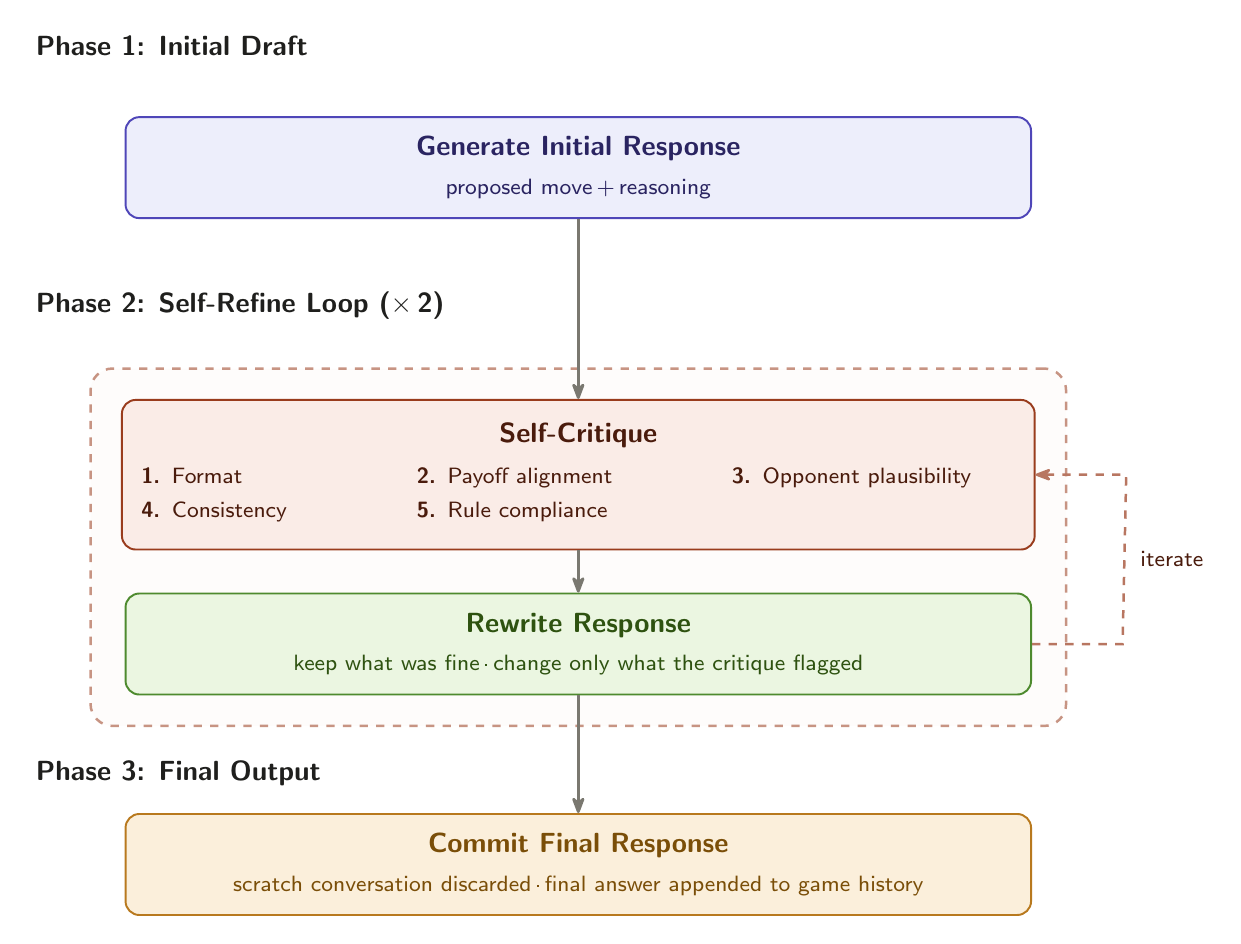
\begin{tikzpicture}[
  font=\sffamily,
  box/.style    ={rounded corners=5pt, draw, line width=0.7pt, align=center, inner sep=7pt},
  draft/.style  ={box, fill=memFill, draw=memLine, text=memText,
                  minimum width=11.5cm, minimum height=1.2cm},
  crit/.style   ={box, fill=rewFill, draw=rewLine, text=rewText,
                  minimum width=11.5cm, minimum height=1.9cm},
  ref/.style    ={box, fill=movFill, draw=movLine, text=movText,
                  minimum width=11.5cm, minimum height=1.2cm},
  final/.style  ={box, fill=borFill, draw=borLine, text=borText,
                  minimum width=11.5cm, minimum height=1.2cm},
  phase/.style  ={text=phaseText, font=\sffamily\bfseries, anchor=west,
                  fill=white, inner sep=3pt},
  flow/.style   ={-{Stealth[round]}, draw=arrowGray, line width=1pt},
  back/.style   ={-{Stealth[round]}, draw=rewLine!70, line width=0.9pt, dashed},
]

% ----- Phase 1: Initial Draft -----
\node[phase] at (-0.1, 1.55) {Phase 1: Initial Draft};
\node[draft] (DRAFT) at (6.9, 0)
  {\textbf{Generate Initial Response}\\[2pt]
   \footnotesize proposed move\,+\,reasoning};

% ----- Phase 2: Self-Refine Loop -----
\node[phase] at (-0.1, -1.75) {Phase 2: Self-Refine Loop ($\times$\,2)};

\node[crit] (CRIT) at (6.9, -3.9)
  {\textbf{Self-Critique}\\[5pt]
   \footnotesize
   \begin{tabular}{@{}p{2.9cm}@{\hspace{0.6cm}}p{3.4cm}@{\hspace{0.6cm}}p{3.6cm}@{}}
     \textbf{1.}\enspace Format &
     \textbf{2.}\enspace Payoff alignment &
     \textbf{3.}\enspace Opponent plausibility \\[3pt]
     \textbf{4.}\enspace Consistency &
     \textbf{5.}\enspace Rule compliance &
   \end{tabular}};

\node[ref] (REF) at (6.9, -6.05)
  {\textbf{Rewrite Response}\\[2pt]
   \footnotesize keep what was fine\,·\,change only what the critique flagged};

% Dashed enclosure for the iterated block
\begin{scope}[on background layer]
  \node[draw=rewLine!55, dashed, rounded corners=8pt, line width=0.9pt,
        fit=(CRIT)(REF), inner sep=11pt, fill=rewFill!18] (LOOPBOX) {};
\end{scope}

% ----- Phase 3: Final Output -----
\node[phase] at (-0.1, -7.7) {Phase 3: Final Output};
\node[final] (FINAL) at (6.9, -8.85)
  {\textbf{Commit Final Response}\\[2pt]
   \footnotesize scratch conversation discarded\,·\,final answer appended to game history};

% ----- Arrows -----
\draw[flow] (DRAFT.south) -- (CRIT.north);
\draw[flow] (CRIT.south)  -- (REF.north);
\draw[flow] (REF.south)   -- (FINAL.north);

% Loop-back arrow on the right side
\coordinate (loopBot) at ($(REF.east)  + (1.15,0)$);
\coordinate (loopTop) at ($(CRIT.east) + (1.15,0)$);
\draw[back] (REF.east) -- (loopBot) -- (loopTop) -- (CRIT.east);

% Label on the loop arrow
\node[font=\sffamily\footnotesize, text=rewText, anchor=west]
  at ($(loopBot)!0.5!(loopTop) + (0.08,0)$) {iterate};

\end{tikzpicture}
\end{document}
